\section{Covers and Hasse diagrams}

If $s, t \in P$, then we say that $t$ covers $s$ or $s$ is covered by $t$, denoted $s \lessdot t$ or $t \gtrdot s$, if $s < t$ and no element $u \in P$ satisfies $s < u < t$. Thus $t$ covers $s$ if and only if $s < t$ and $[s, t] = {s, t}$. A locally finite poset $P$ is completely determined by its cover relations. The Hasse diagram of a finite poset $P$ is the graph whose vertices are the elements of $P$, whose edges are the cover relations, and such that if $s < t$ then $t$ is drawn “above” $s$ (i.e., with a higher vertical coordinate). \ref{fig:stanley:3-1} shows the Hasse diagrams of all posets up to isomorphism) with at most four elements. Some care must be taken in “recognizing” posets from their Hasse diagrams. For instance, the graph 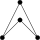
\includegraphics{fig/stanley/3-1:a} is a perfectly valid Hasse diagram, yet appears to be missing from \ref{fig:stanley:3-1}. We trust the reader will resolve this anomaly. Similarly, why does the graph 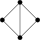
\includegraphics{fig/stanley/3-1:b} not appear above? \ref{fig:stanley:3-2} illustrates the Hasse diagrams of some of the posets considered in \ref{ex:poset:def}. \cite{Stanley:2011:ECV:2124415}

\begin{figure}
	\centering
	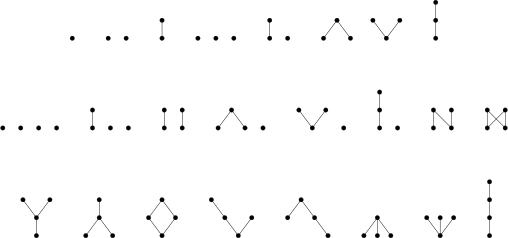
\includegraphics[width=\textwidth]{fig/stanley/3-1}
	\caption{\label{fig:stanley:3-1} The posets with at most four elements. \cite{Stanley:2011:ECV:2124415}}
\end{figure}


\begin{figure}
	\centering
	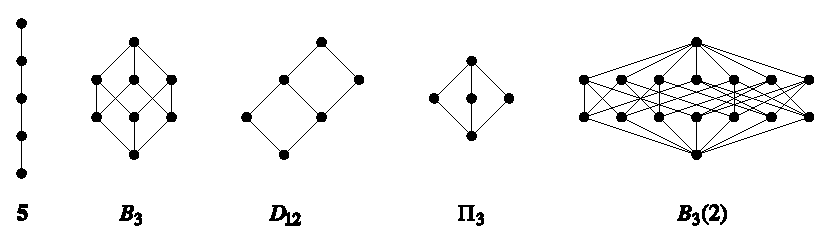
\includegraphics[width=\textwidth]{fig/stanley/3-2}
	\caption{\label{fig:stanley:3-2} Some examples of posets. \cite{Stanley:2011:ECV:2124415}}
\end{figure}